\section{CONAE y aplicaciones}
\subsection{Plan espacial nacional}
\begin{frame}{\secname : \subsecname}
  \begin{figure}
    \centering
    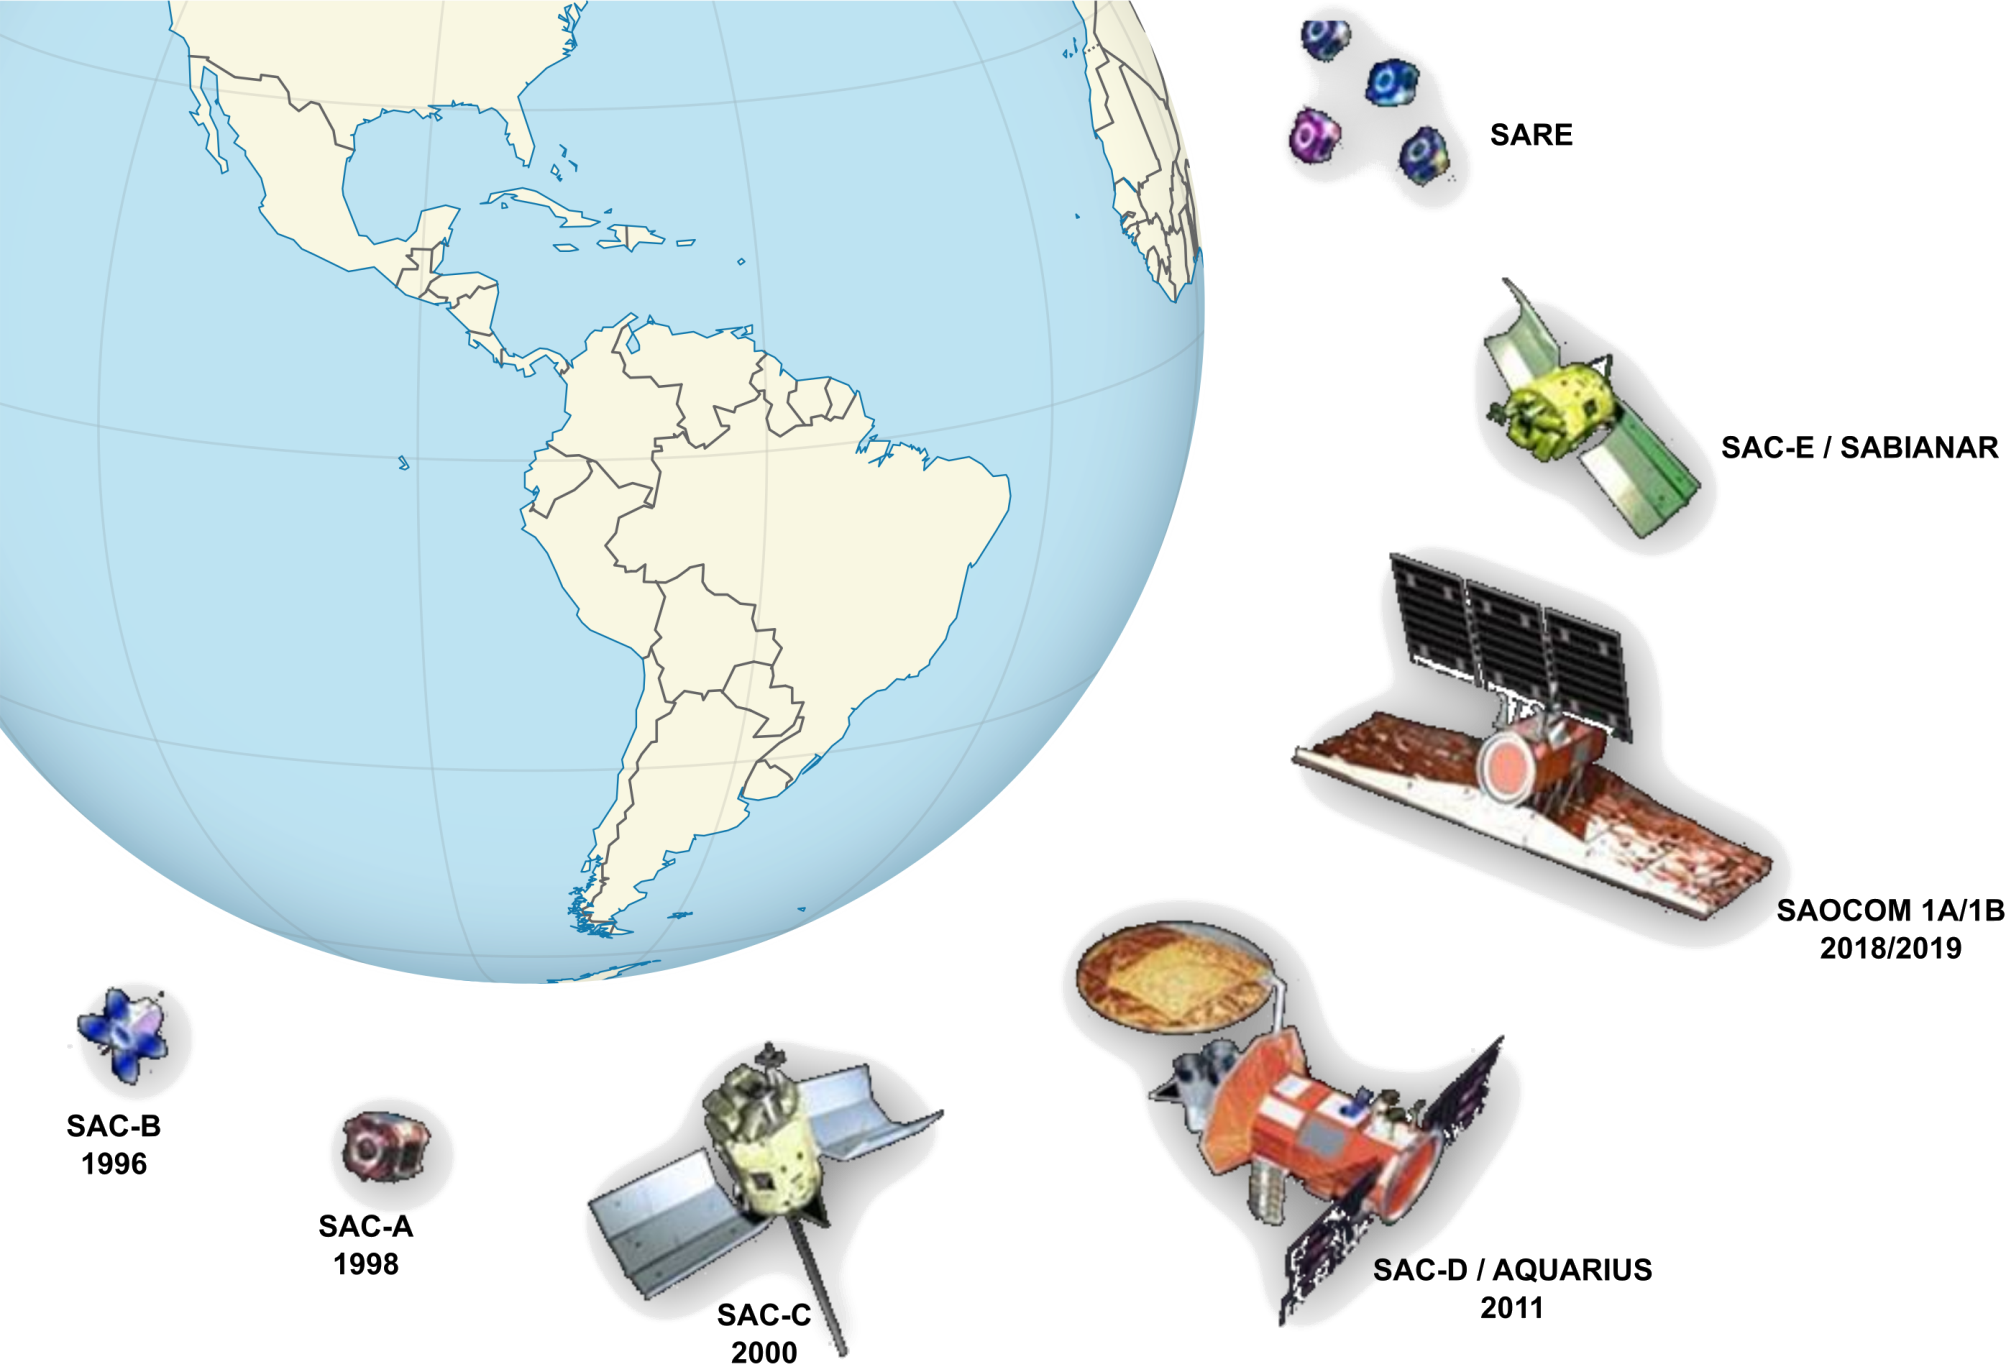
\includegraphics[width=0.65\textwidth]{fig:plan}
    \caption{Satélites del plan espacial nacional.}
    \label{}
  \end{figure}
\end{frame}
%--- Next Frame ---%

\subsection{Aplicaciones de la teledetección}

\begin{frame}{\secname : \subsecname}
  \begin{figure}
    \centering
    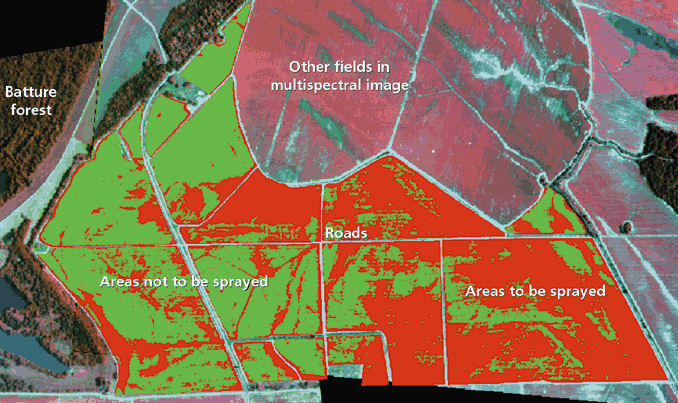
\includegraphics[width=0.65\textwidth]{fig:app-cultivo.jpg}
    \caption{Mapeo de áreas afectadas por plagas, Delta del Mississippi, USA. \emph{Fuente: Environmental Health Perspectives, Volume 108 (3), March 2000}.}
    \label{}
  \end{figure}
\end{frame}
%--- Next Frame ---%

\begin{frame}{\secname : \subsecname}
  \begin{figure}
    \centering
    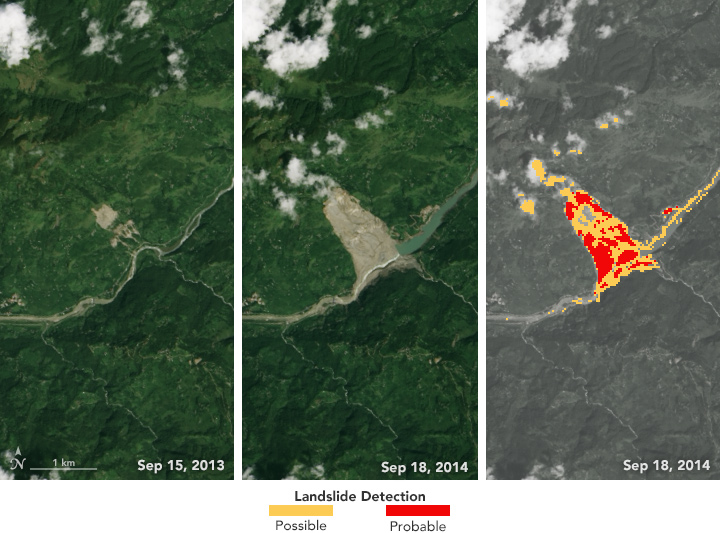
\includegraphics[width=0.55\textwidth]{fig:app-cambio.jpg}
    \caption{Detección de un deslizamiento utilizando imágenes Landsat 8, Nepal. \emph{Fuente: Automating the Detection of Landslides, NASA, July 6, 2016}.}
    \label{}
  \end{figure}
\end{frame}
%--- Next Frame ---%

\begin{frame}{\secname : \subsecname}
  \begin{figure}
    \centering
    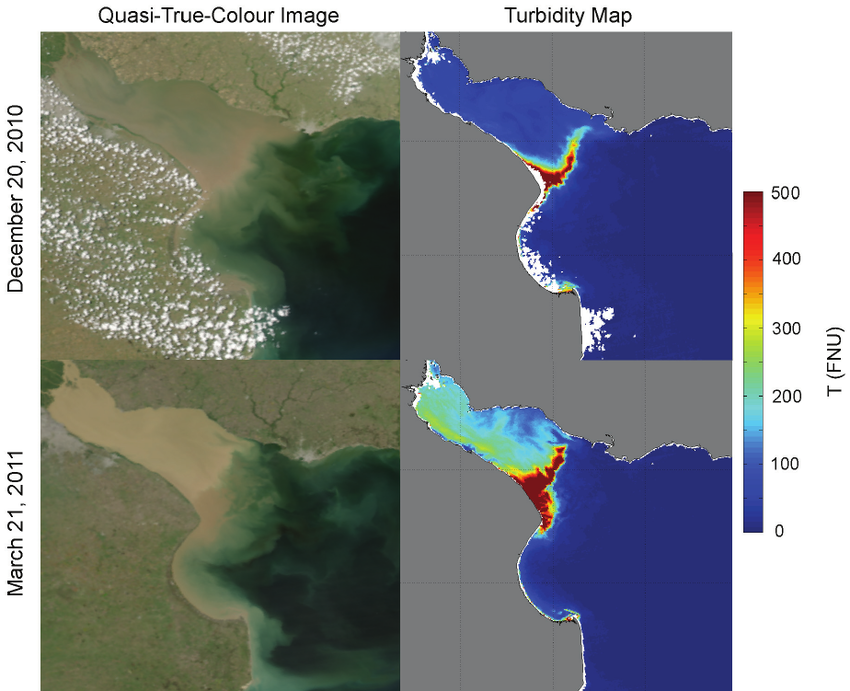
\includegraphics[width=0.45\textwidth]{fig:app-turb.png}
    \caption{Cálculo de turbidez para la zona del Río de la Plata, Argentina/Uruguay. \emph{Fuente: CALIBRATION AND VALIDATION OF AN ALGORITHM FOR REMOTE SENSING OF TURBIDITY OVER LA PLATA RIVER ESTUARY, ARGENTINA}}
    \label{}
  \end{figure}
\end{frame}
%--- Next Frame ---%

\begin{frame}{\secname : \subsecname}
  \begin{figure}
    \centering
    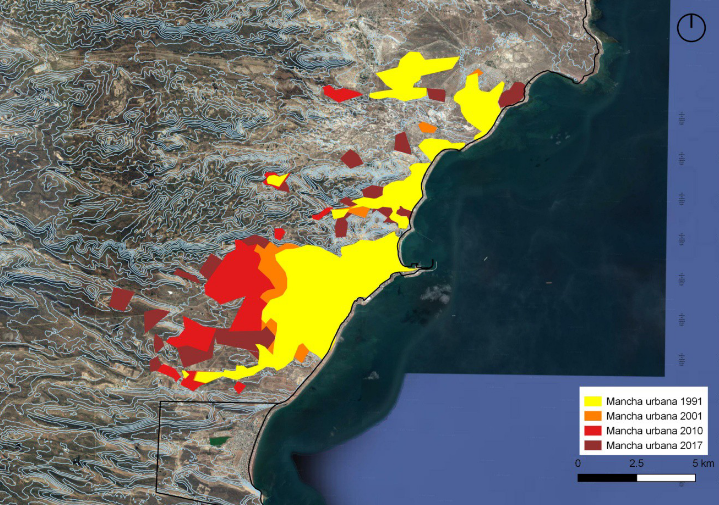
\includegraphics[width=0.60\textwidth]{fig:app-exp.png}
    \caption{Expansión urbana 1990-2017, Comodoro Rivadavia, Chubut, Argentina. \emph{Fuente: ANÁLISIS DE
EXPANSIÓN URBANA Comodoro Rivadavia 2017}}
    \label{}
  \end{figure}
\end{frame}
%--- Next Frame ---%

\begin{frame}{\secname : \subsecname}
  \begin{figure}
    \centering
    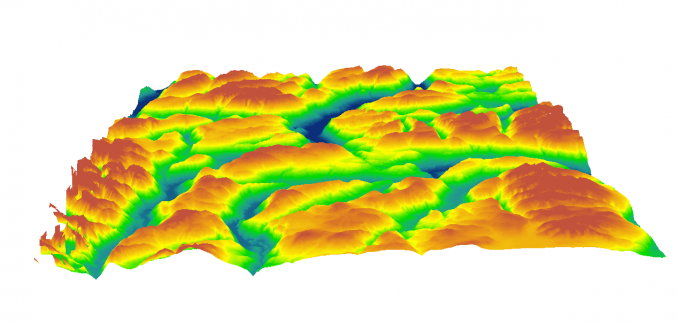
\includegraphics[width=0.60\textwidth]{fig:app-dem.png}
    \caption{Modelo digital de elevación de 2014. \emph{Fuente: NASA SRTM}}
    \label{}
  \end{figure}
\end{frame}
%--- Next Frame ---%



\begin{frame}{\secname : \subsecname}
Muchas gracias.
\end{frame}
%--- Next Frame ---%
